\chapter{Agile Project Management}
\label{chapter:introduction}

    During the development of our smart flight check-in kiosk, we adopted agile project management and use “Scrum Approach” to manage the iterative development. 
    The whole Scrum process is roughly divided into the following three phases:
    \begin{enumerate}
        \item \textbf{Plan and Design:} In this part, we selected our Scrum Master, wrote user story, product backlog, and completed prototype design. 
        \item \textbf{Development phase:} In this part, we followed a series of Sprint Cycles, where each cycle developed a version of working software during 2 weeks.
        \item \textbf{Product release:} In this part, we checked our project against the requirements and wrapped up our project by writing reports, user manuals, etc.
    \end{enumerate}
    
    \begin{figure}[H]
    \centering
    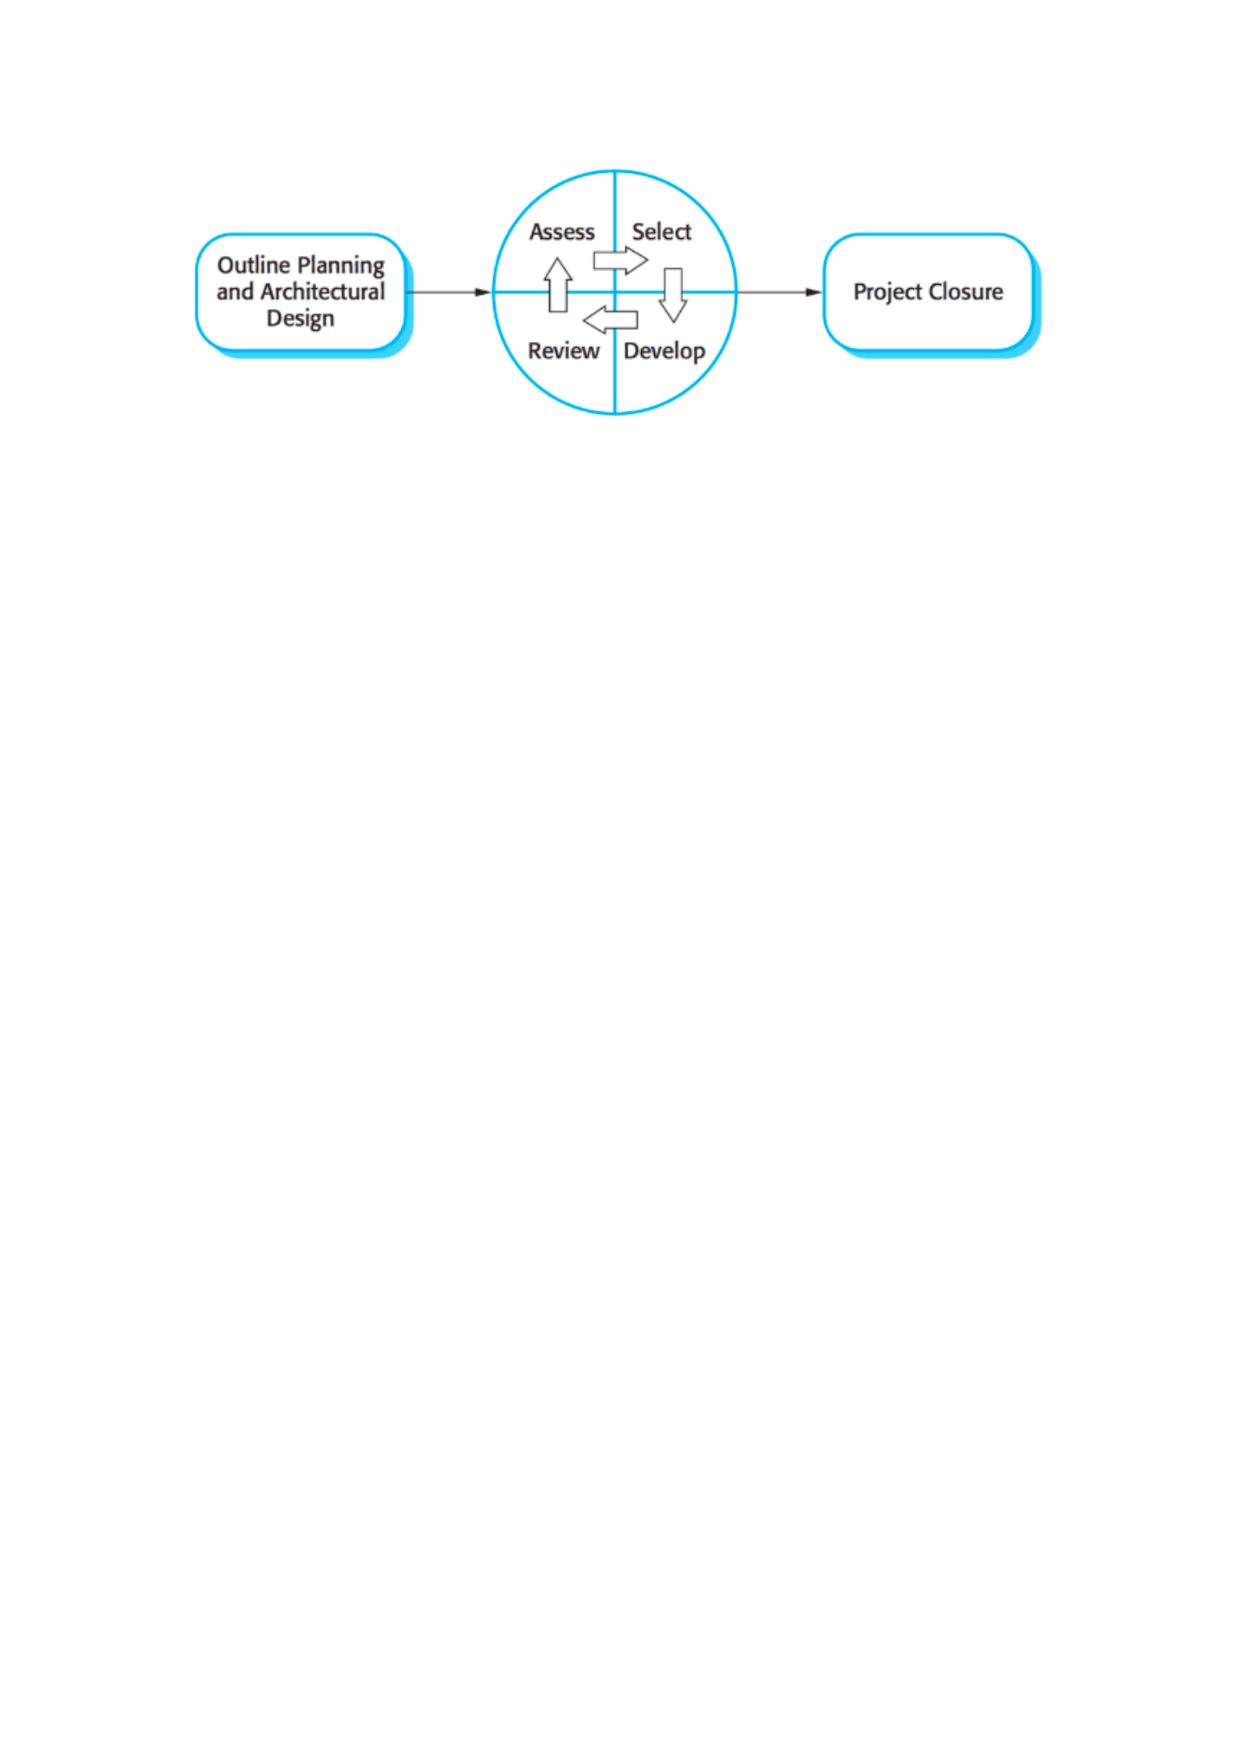
\includegraphics[width=0.7\linewidth]{figures/c1/sprint.pdf}
    \caption{Sprint Cycle}
    \label{c1_1}
    \end{figure}

\section{First phase: Plan and Design}    
\subsection{Project planning and scheduling}
\subsection{}
